 \chapter{Route Page:}
 The (Audio) Route Page is used to send the audio of a specific MD track to a selected output. \\
 \\\textbf{[ Encoder 1]} can be used to select the audio output to MD external outputs C -> F.\\

\fbox{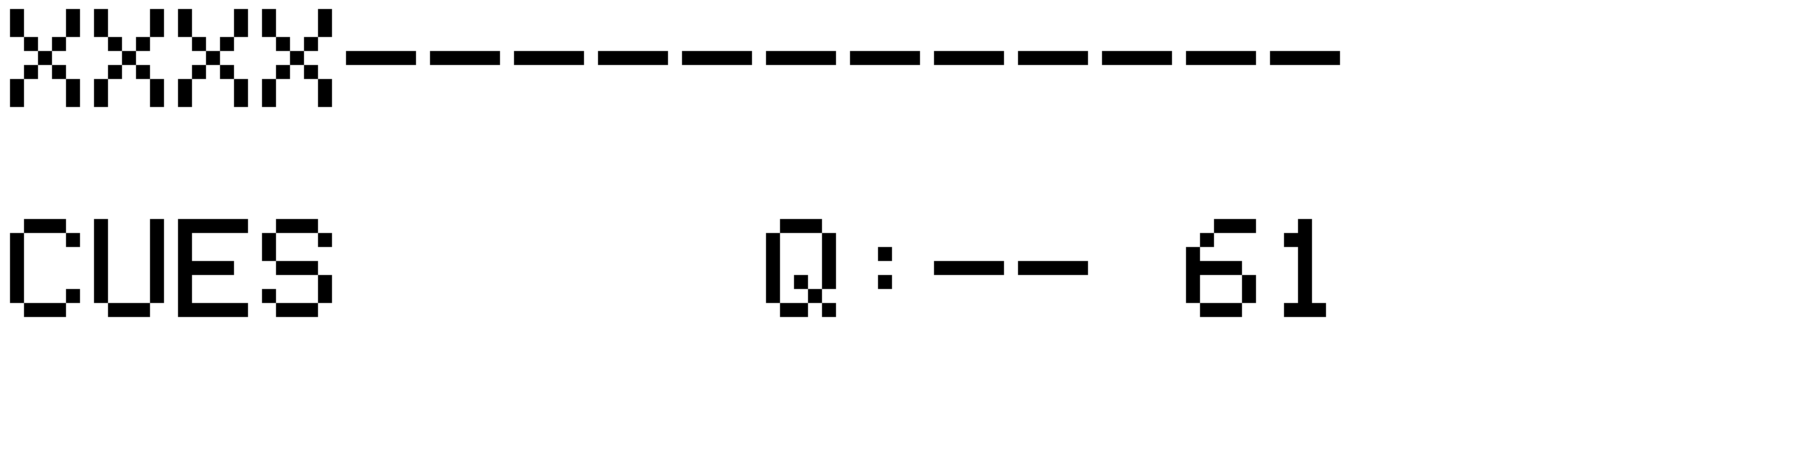
\includegraphics[scale=.40]{cue_page.png}}\\\\
 \textit{The Route Page is accessible from the PageSelect page.}
  \section{Encoder Assignment:}
 \begin{itemize}
 	\item \textbf{[ Encoder 1 ]: } Output Selection
 	\item \textbf{[ Encoder 2 ]: } --
 	\item \textbf{[ Encoder 3 ]: } Quantization
 	\item \textbf{[ Encoder 4 ]: } --
 \end{itemize}
  The trigger interface used to toggle the output of selected tracks, between Main Outputs and the chosen external output.
 \section{Quantization Modes:}
 Quantization modes are used to control the behaviour of the cue operations and allow for cue events to be musically timed.\\
 \\
 When a numerical quantization value is chosen the selected track’s cue will be toggled on the next specified multiple of the step-count.
 \begin{itemize}
\item --: No quantization.
\item 02: Toggle cue on next possible 2nd step
\item 04: Toggle cue on next possible 4th step
\item 08: Toggle cue on next possible 8th step 
\item 16: Toggle cue on next possible 16th step 
\item 32: Toggle cue on next possible 32th step 
\item 64: Toggle cue on next possible 64th step
 \end{itemize}
 
 